\documentclass[onecolumn]{article}
%\usepackage{url}
%\usepackage{algorithmic}
\usepackage[a4paper]{geometry}
\usepackage{datetime}
\usepackage{hyperref}
\usepackage[margin=2em, font=small,labelfont=it]{caption}
\usepackage{graphicx}
\usepackage{mathpazo} % use palatino
\usepackage[scaled]{helvet} % helvetica
\usepackage{microtype}
\usepackage{amsmath}
\usepackage{subfigure}
\usepackage{listings}
\usepackage{float}
\usepackage{xcolor} %red, green, blue, yellow, cyan, magenta, black, white
\usepackage{graphicx}
\usepackage[font=small,labelfont=bf]{caption}
\renewcommand{\thefigure}{\arabic{section}.\arabic{figure}}
\graphicspath{ {pictures/} }
\definecolor{mygreen}{RGB}{28,172,0} % color values Red, Green, Blue
\definecolor{lightgray}{gray}{0.9}
\definecolor{mylilas}{RGB}{170,55,241}
\newcommand{\inlinecode}[2]{\colorbox{lightgray}{\lstinline[language=#1]$#2$}}


% Letterspacing macros
\newcommand{\spacecaps}[1]{\textls[200]{\MakeUppercase{#1}}}
\newcommand{\spacesc}[1]{\textls[50]{\textsc{\MakeLowercase{#1}}}}
\newcommand{\inline}[1]{\colorbox{lightgray}{\lstinline[basicstyle=\ttfamily\color{brown}]|#1|}}

\title{\spacecaps{Lab report: Lab 5 }\\
Radiation balance of the Earth\\\normalsize \spacesc{Modeling of Physical Systems} }

\author{Patryk Gałczyński}
%\date{\today\\\currenttime}
\date{\today}


\begin{document}
\lstset{language=Matlab,%
    %basicstyle=\color{red},
    %breaklines=true,%
    morekeywords={matlab2tikz},
    keywordstyle=\color{blue},%
    morekeywords=[2]{1}, keywordstyle=[2]{\color{black}},
    identifierstyle=\color{black},%
    stringstyle=\color{mylilas},
    commentstyle=\color{mygreen},%
    showstringspaces=false,%without this there will be a symbol in the places where there is a space
    numbers=left,%
    numberstyle={\small \color{black}},% size of the numbers
    numbersep=9pt, % this defines how far the numbers are from the text
    emph=[1]{for,end,break},emphstyle=[1]\color{red}, %some words to emphasise
    %emph=[2]{word1,word2}, emphstyle=[2]{style},    
}

\maketitle


\section{Aim}
\large
The aim of this laboratory was to simulate, visualize and analyze Earth radiation balance leading to two models of Earth temperature (one omitting atmosphere influence and one including it). An additional goal was to find relationship between solar constant and mean Earth temperature, and also check how glaciations mechanism changes model behavior.


\section{Methods}
For the laboratory purpose various tools and methods were selected to achieve good simulation results and easy in depth analysis. For mean Earth temperature calculation, energy balance equations has been used. This report considers two main models: Earth with and without atmosphere, resulting in very different sets of energy balance equations.

\section{Simulation description and Results}
\subsection{Simulation models}
To simulate Earth radiation balance phenomena two different models were used.
\begin{enumerate}
	\item Model 1 - without atmosphere \\
      This fairly simple models assumes that there is no atmosphere around the Earth. This very simplifies energy balance equation. It is given in form:
      \begin{equation}
          P_{Sol} = S \cdot \frac{Pow_z}{4} \cdot (1 - A)
      \end{equation}
      \begin{equation}
          P_{Earth} = \sigma \cdot T^4 \cdot Pow_z
      \end{equation}
      Assuming that power of solar radiation arriving to the Earth is equal to power of radiation emitted from Earth:
      \begin{equation}
          P_{Earth} = P_{Sol}
      \end{equation}
      Because point of interest of this part is to get mean Temperature, after substitution, this equation could be presented as:
      \begin{equation}
          T = \sqrt[4]{\frac{S \cdot (1 - A)}{4 \cdot \sigma}}
      \end{equation}
      Where:
      \begin{itemize}
          \item S = $1366 \frac{W}{m^2}$ - Solar constant
          \item A = $0.3$ - Mean albedo of the Earth surface
          \item $\sigma$ = $5.67 \cdot 10^{-8} \frac{W}{m^2K^4}$ - Stefan Boltzmann constant
      \end{itemize}
      To calculate that, simple MATLAB script were written:
      \begin{lstlisting}[language=Matlab,frame=single,label={lst:autocorr},breaklines=true,caption={Mean Earth temperature without atmosphere calculation script}]
A = 0.30;                       % albedo
S = 1366;                       % W/m^2
sigma = 5.67 * (10^-8);         % W/m^2K^4
T4 = S * (1 - A) / (sigma * 4); % K^4
T = T4 ^ (1/4);                 % K
output = [
    'Mean earth temperature without atmosphere in:', newline, ...
    '  Kelvins: ', num2str(T), ' K' newline, ...
    '  Celsius: ', num2str(T - 273.15), ' deg of C' newline
];
disp(output);
      \end{lstlisting}
      Its execution results in:
      \begin{lstlisting}[language=Matlab,frame=single,label={lst:autocorr},breaklines=true,caption={Mean Earth temperature without atmosphere calculation script execution}]
>> mean_temp
Mean earth temperature without atmosphere in:
  Kelvins: 254.8158 K
  Celcius: -18.3342 deg of C
      \end{lstlisting}
    \newpage
    \item Model 2 - with atmosphere \\
      This time, model includes atmosphere influence at Earth radiation balance. Following equations describe mentioned model:
      \begin{equation}
      	(-t_a)(1-a_s)\frac{S}{4} + c(T_s - T_a) + \sigma T_S^4 (1-a'_a) - \sigma T_a^4 = 0
      \end{equation}
      \begin{equation}
      	-(1 - a_a - t_a + a_s t_a) \frac{S}{4} - c(T_s - T_a) - \sigma T_s^4 (1 - t'_a - a'_a) + 2 \sigma T_a^4 = 0
      \end{equation}
      where:
      \begin{itemize}
          \item S = $1366 \frac{W}{m^2}$ - Solar constant
          \item $a_a$ = $0.30$ - albedo of the atmosphere (short waves)
          \item $a'_a$ = $0.31$ - albedo of the atmosphere (long waves)
          \item $a_s$ = $0.19$ - albedo of the surface
          \item $t_a$ = $0.53$ - transmission of the atmosphere (short waves)
          \item $t'_a$ = $0.06$ - transmission of the atmosphere (long waves
          \item $c$ = $2.7 \frac{W}{m^2K}$ - heat transfer coefficient
          \item $\sigma$ = $5.67 \cdot 10^{-8} \frac{W}{m^2K^4}$ - Stefan Boltzmann constant
      \end{itemize}
      It can be easily spotted that these equations are non-linear. To find values of $T_s$ (mean temperature of surface) and $T_a$ (mean temperature of atmosphere), MATLAB \inline{fsolve(fun,x0)} function, which is capable of solving non linear equations passed as function \inline{fun} and it starts at \inline{x0}, were used. \\
      Following MATLAB script has been created for this purpose:
      \begin{lstlisting}[language=Matlab,frame=single,label={lst:autocorr},breaklines=true,caption={Mean Earth temperature with atmosphere calculation script}]
% declare constants as globals so heatfun function can use it
global ta ta_p as aa aa_p S c sigma
% assign values to constants
ta = 0.53;       
ta_p = 0.06;
as = 0.19;
aa = 0.30;
aa_p = 0.31;
S  = 1366;              % W/m^2
c  = 2.7;               % Wm-2K-1
sigma = 5.67 * (10^-8); % W/m^2K^4
Ts = 273;               % start with 0 deg. of Celsius
Ta = 273;               % surface and atmosphere temp
Xp = [Ts Ta];

% solve equations from heatfun using fsolve 
X = fsolve(@heatfun, Xp);

% and print results
output = [
    'Mean earth temperature with atmosphere in:', newline, ...
    '  Kelvins: ', num2str(X(1)), ' K' newline, ...
    '  Celsius: ', num2str(X(1) - 273.15), ' deg of C', newline ...
    'Mean atmosphere temperature in:', newline, ...
    '  Kelvins: ', num2str(X(2)), ' K' newline, ...
    '  Celsius: ', num2str(X(2) - 273.15), ' deg of C' newline
];
disp(output);

% heatfun function using defined equations
function F = heatfun(x)
    global ta as aa S c sigma ta_p aa_p
    F = [ -1 * ta * (1 - as) * (S/4) + ...
            c * (x(1) - x(2)) + ...
            sigma * (x(1) ^ 4) * (1 - aa_p) ...
            - sigma * (x(2) ^ 4);
          -1 * (1 - aa - ta + as*ta) * S / 4 ...
            - c * (x(1) - x(2)) ...
            - sigma * (x(1) ^ 4) * (1 - ta_p - aa_p) ...
            + 2 * sigma * x(2)^4;
        ];
end
      \end{lstlisting}
      \newpage
	  And the result of execution of such script is:
      \begin{lstlisting}[language=Matlab,frame=single,label={lst:autocorr},breaklines=true,caption={Mean Earth temperature with atmosphere calculation script execution}]
Mean earth temperature with atmosphere in:
  Kelvins: 285.992 K
  Celsius: 12.842 deg of C
Mean atmosphere temperature in:
  Kelvins: 248.5215 K
  Celsius: -24.6285 deg of C
      \end{lstlisting}
\end{enumerate}
\subsection{Compassion of results}
In two simulated models Earth temperature differs for about 30 degrees, yet they are in the same order of magnitude, which is good. According to NASA (\url{https://climate.nasa.gov/vital-signs/global-temperature/}), current mean Earth temperature is $0.9^{o}C$ which is somewhere in the middle of our models results. This still can be considered as a success regarding simpleness of provided models.

\subsection{Relationship between solar constant and mean temp result}
To check such relationship the following MATLAB script were written (to save space boiler-plate code as constants definition were erased)
\begin{lstlisting}[language=Matlab,frame=single,label={lst:autocorr},breaklines=true,caption={Correlation between solar constant and mean temperature script}]
...
% check solar constant from 0.8 of S to 1.2 of S
old_s = 1366
s_vector = round(0.8 * old_s):round(1.2*old_s);
temp_e_vector = [];
temp_a_vector = [];
for i = s_vector
    S = i;
    Xp = [Ts Ta];
    X = fsolve(@heatfun, Xp);
    temp_e_vector = [temp_e_vector X(1) - 273.15];
    temp_a_vector = [temp_a_vector X(2) - 273.15]; 
end





% plot results
figure;
plot(s_vector, temp_e_vector);
title('Relationship between solar constant and mean earth temp result');
xlabel('Solar constant [W/m^2]');
ylabel('Mean Earth temp [deg. of C]');

figure;
plot(s_vector, temp_a_vector);
title('Relationship between solar constant and mean atmoshpere temp result');
xlabel('Solar constant [W/m^2]');
ylabel('Mean Atm temp [deg. of C]');
...
\end{lstlisting}

Execution of this script results in two charts: \\
\noindent\makebox[\textwidth]{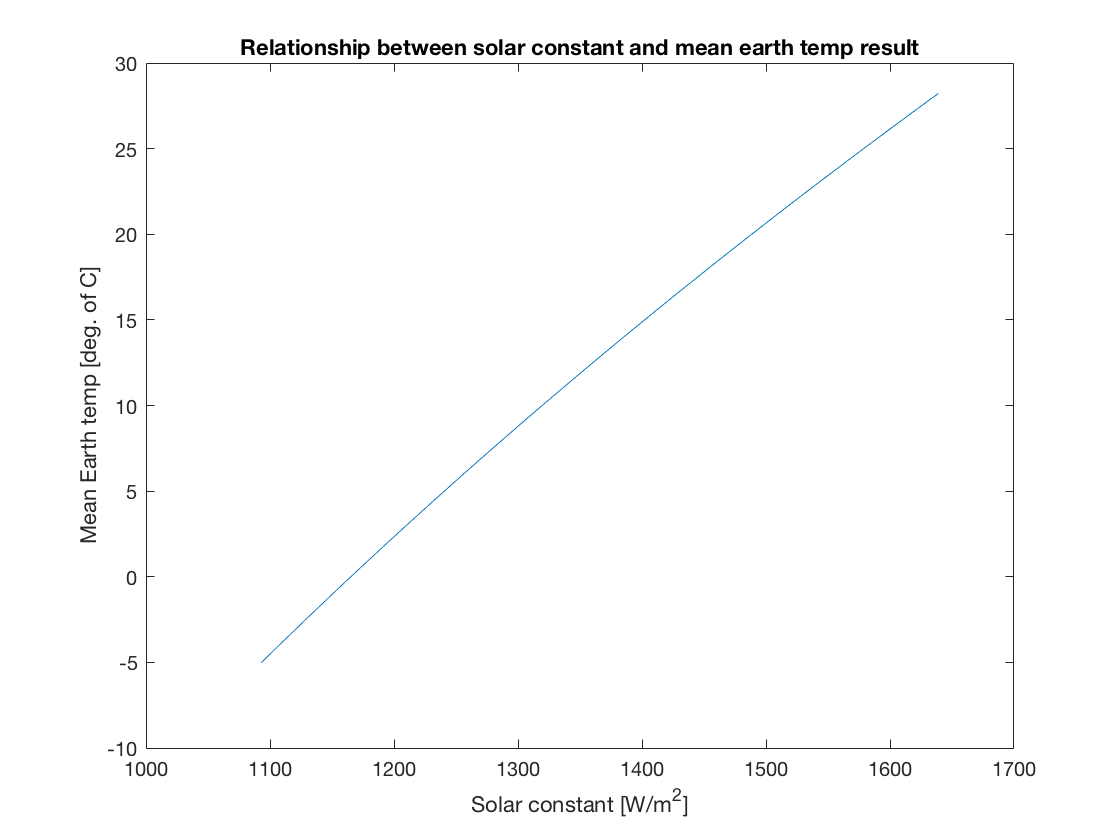
\includegraphics[scale=0.3]{relationship_earth}}
\noindent\makebox[\textwidth]{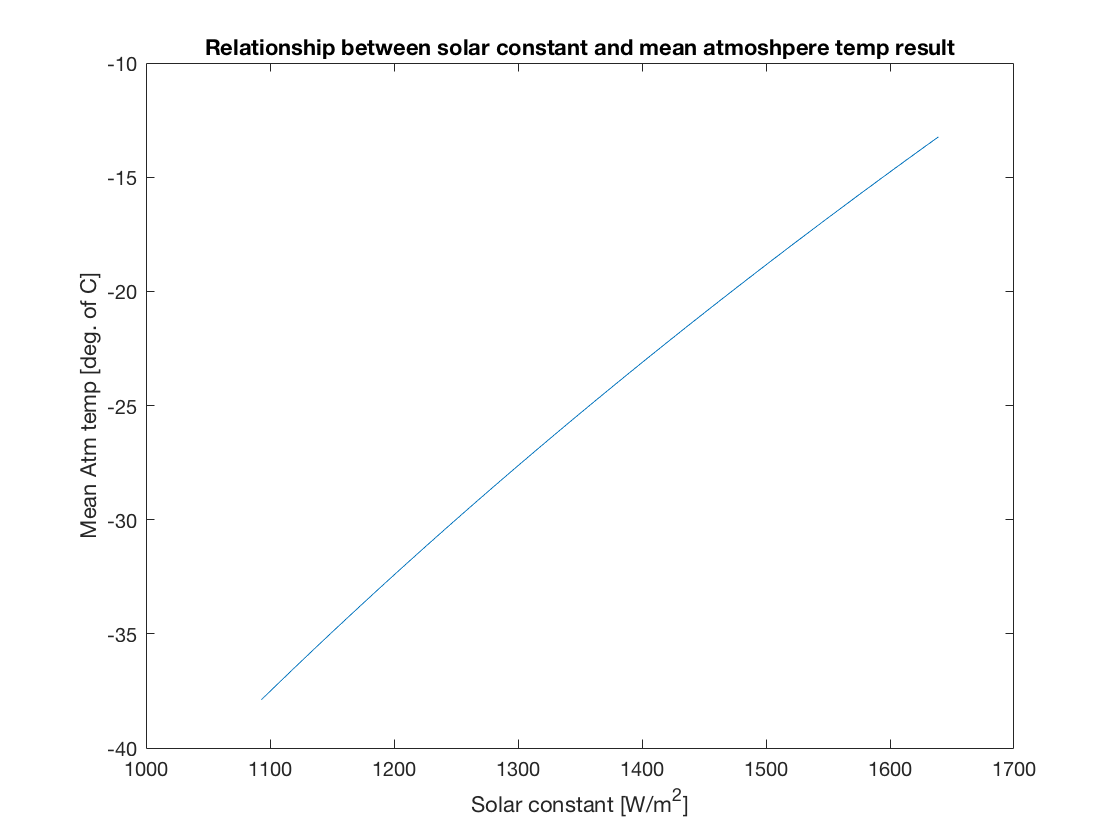
\includegraphics[scale=0.3]{relationship_atm}}

It is noticeable, that this relationship is almost linear.

\newpage
\subsection{Extend model 2 with glaciations mechanism}
To embed glaciations mechanism in model of mean Earth temperature including atmosphere, one simple change is needed as shown in code below:

\begin{lstlisting}[language=Matlab,frame=single,label={lst:autocorr},breaklines=true,caption={Correlation between solar constant and mean temperature script}]
...
s_vector = round(0.8 * oldS):round(1.2*oldS);
temp_e_vector = [];
temp_a_vector = [];
for i = s_vector
    S = i;
    Xp = [Ts Ta];
    X = fsolve(@heatfun, Xp);
    temp_e_vector = [temp_e_vector X(1) - 273.15];
    temp_a_vector = [temp_a_vector X(2) - 273.15];
    
    % check whether surface is covered with ice
    if X(1) - 273.15 < -5
        % albedo for snow
        as = 0.8; 
    else
        % normal albedo
        as = 0.19;
    end
end
...
\end{lstlisting}
This approach assumes that, surface is being covered with ice, if its temperature is below $-5^o C$. Running code with presented changes gives the following results:

\noindent\makebox[\textwidth]{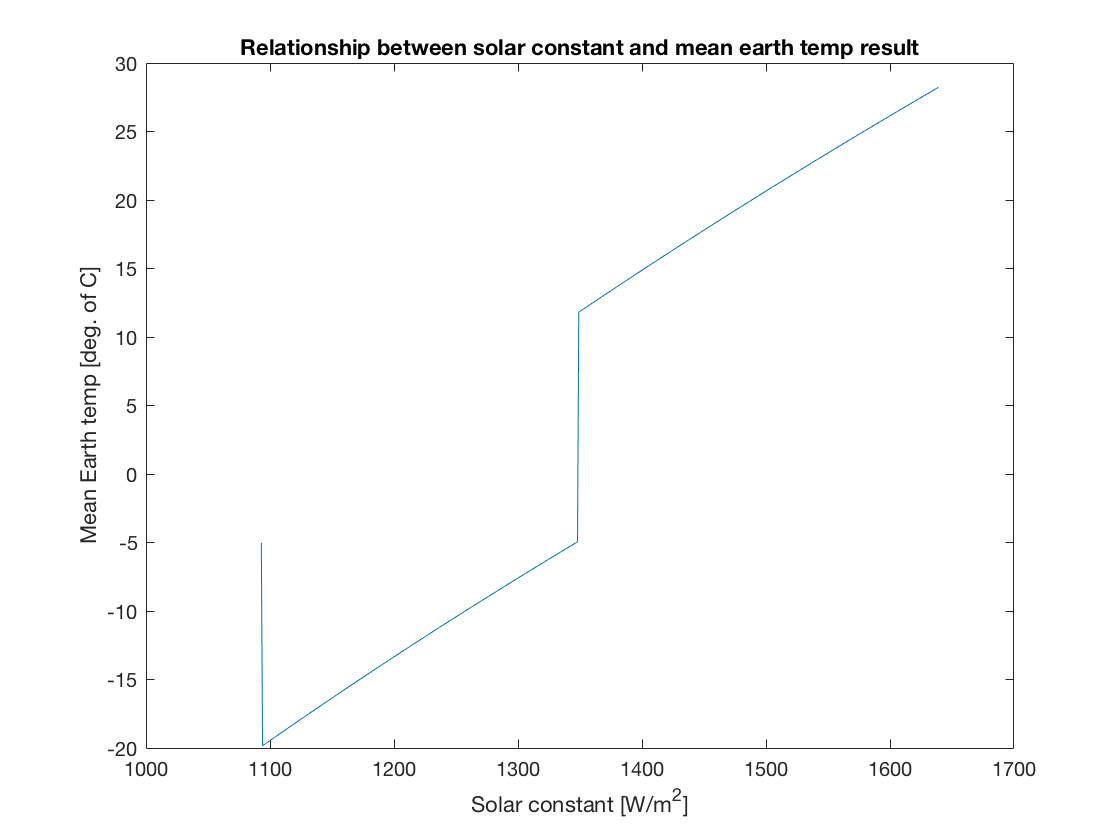
\includegraphics[scale=0.3]{relationship_earth_ice}}
\noindent\makebox[\textwidth]{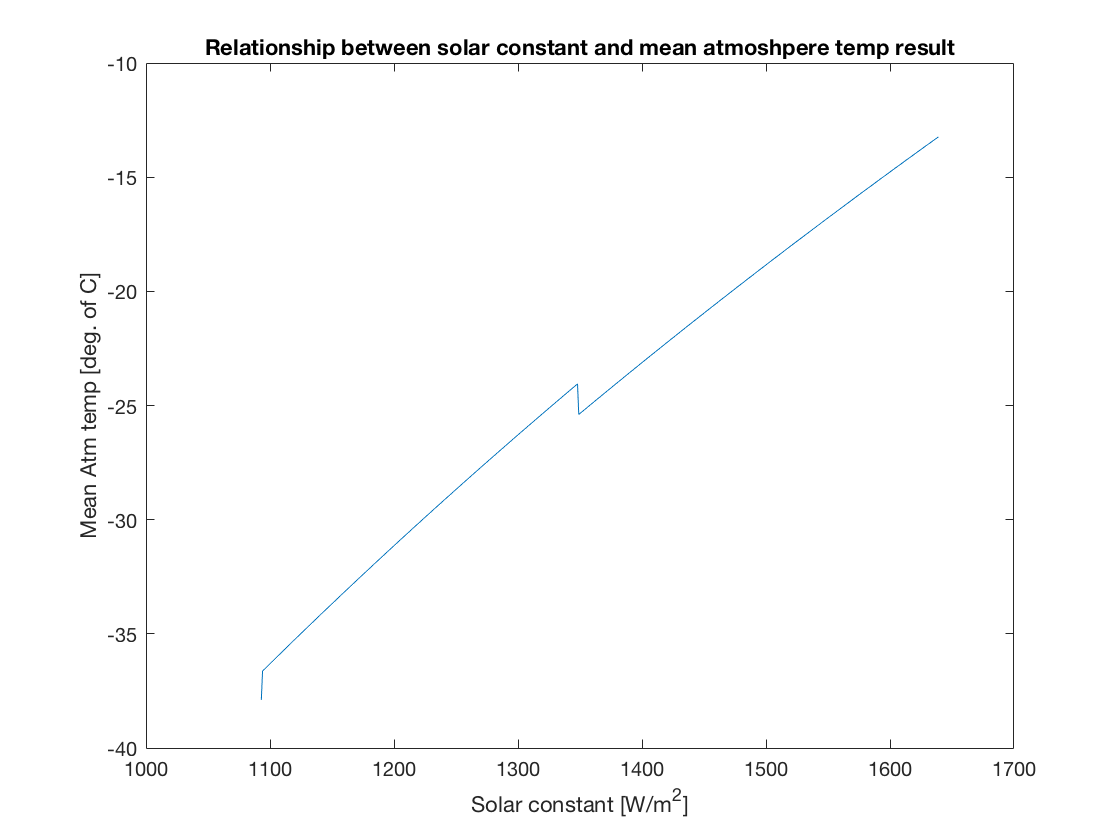
\includegraphics[scale=0.3]{relationship_atm_ice}}

\subsection{Glaciations mechanism results}
From presented pictures, it can be concluded that, when ice mets and albedo is getting much lower (from $0.8$ to $0.19$), rapid temperature grow is observable in Earth temperature. However, in atmospheric chart it is examinable that while Earth surface temperature is growing fast, atmosphere temperature drops a bit. This may be due to much higher earth radiation absorption rate when albedo changes? 


\section{Conclusion}
This report covered two simple models of calculating mean Earth temperature, including and excluding atmosphere impact. Obtained results are satisfiable and accurate, as the delta between these two is relatively small. Also, comparing outcome of these two models and real world data provided by Space Agency, it is withing same order of magnitude, which suggests that these models are correct.
Last but not least, model including atmosphere has been extended with glaciations mechanism, which shown how surface type and its albedo is important in radiation balance model. 
\end{document}
